\subsection{L'ordonanceur (SCHEDULER)}
\label{subsec:scheduler}
L'ordonanceur est une structure de données qui contient les tâches à exécuter. Il se
matérialise par une structure contenant quatre éléments : le nombre de tâches en cours
d'exécution (\texttt{length}\footnoteref{footnote:ref_async_h}), l'indice de la tâche
actuellement en cours d'exécution (\texttt{current\_idx}\footnoteref{footnote:ref_async_h}),
le nombre de tâches exécutées depuis le dernier tour de boucle (\texttt{nbr\_has\_run\_task}
\footnoteref{footnote:ref_async_h}), un tableau de pointeurs de tâches (\texttt{tasks}
\footnoteref{footnote:ref_async_h}) et un tableau de booléens indiquant quels sont les pointeurs
du tableau \texttt{tasks} faisant référence à des tâches en cours d'exécution (\texttt{running}
\footnoteref{footnote:ref_async_h}). L'ordonanceur gère également la zone mémoire allouée dans
le tas pour les tâches. Il ne peut gérer qu'un nombre limité de tâches définie par la constante
\texttt{MAX\_TASKS\_NBR}\footnoteref{footnote:ref_async_h} et vaut par défaut 50. Là aussi, si
plus (ou moins) de tâches seront exéctutées en parallèle, il est nécessaire de redéfinir cette
constante en conséquence.

\begin{figure}[h]
    \centering
    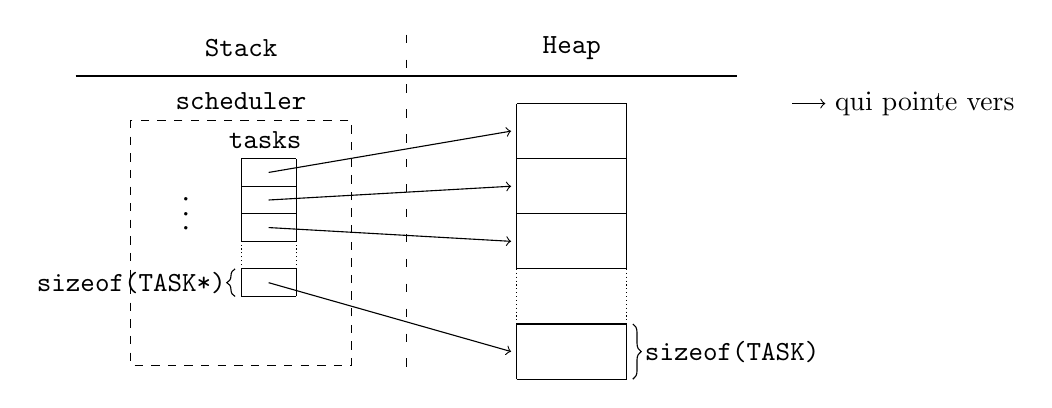
\begin{tikzpicture}[yscale=0.70, xscale=1.4]
        % \draw[help lines] (-6,-3) grid (0, 3);

        \draw node at (-4.5, 3) {\texttt{Stack}};
        \draw node at (-1.5, 3) {\texttt{Heap}};

        \draw (-6, 2.5) -- (0, 2.5);
        \draw[loosely dashed] (-3, 3.25) -- (-3, -3);

        \draw node at (-4.5, 2.05) {\texttt{scheduler}};

        \draw node[anchor=south west] at (-4.7, 1) {\texttt{tasks}};
        \draw[step=0.5] (-4.5, -0.5) grid (-4.0,  1);
        \draw[step=0.5] (-4.5, -1.5) grid (-4.0, -1);
        \draw[densely dotted] (-4.5, -1) -- (-4.5, -0.5);
        \draw[densely dotted] (-4.0, -1) -- (-4.0, -0.5);

        \draw node[rotate=90] at (-5.0, 0) {\texttt{...}};

        % \draw[dashed] (-5.5, 2.25) -- (-3.5, 2.25) -- (-3.5, -2.75) -- (-5.5, -2.75) -- cycle;
        \draw[dashed] (-5.5, 1.7) rectangle (-3.5, -2.75);

        \draw (-2, +2) grid (-1, -1);
        \draw (-2, -2) grid (-1, -3);
        \draw[densely dotted] (-2, -1) -- (-2, -2);
        \draw[densely dotted] (-1, -1) -- (-1, -2);

        \draw[->] (-4.25, +0.75) -- (-2.05, +1.5);
        \draw[->] (-4.25, +0.25) -- (-2.05, +0.5);
        \draw[->] (-4.25, -0.25) -- (-2.05, -0.5);
        \draw[->] (-4.25, -1.25) -- (-2.05, -2.5);

        \draw [decorate,decoration={brace,amplitude=3pt,mirror,raise=0.5ex}]
        (-4.5, -1) -- (-4.5, -1.5) node[midway, anchor=east, xshift=-2]{\texttt{sizeof(TASK*)}};

        \draw [decorate,decoration={brace,amplitude=3pt,raise=0.5ex}]
        (-1, -2) -- (-1, -3) node[midway, anchor=west, xshift=3]{\texttt{sizeof(TASK)}};

        \draw[->] (0.5, 2) -- (0.8, 2) node[right] {qui pointe vers};

    \end{tikzpicture}
    \caption{L'agencement des tâches dans le tas et leur lien avec l'ordonanceur}
\end{figure}